\documentclass[10pt,twocolumn,letterpaper]{article}

%%%%%%%%% PAPER TYPE  - PLEASE UPDATE FOR FINAL VERSION
%\usepackage[review]{cvpr24}      % To produce the REVIEW version
%\usepackage{cvpr}              % To produce the CAMERA-READY version
\usepackage[pagenumbers]{cvpr} % To force page numbers, e.g. for an arXiv version
\usepackage{bm}

% updated April 2002 by Antje Endemann
% Based on CVPR 07 and LNCS, with modifications by DAF, AZ and elle, 2008 and AA, 2010, and CC, 2011; TT, 2014; AAS, 2016; AAS, 2020; TH, 2022

\usepackage{graphicx}
\usepackage{tikz}
% The "axessiblity" package can be found at: https://ctan.org/pkg/axessibility?lang=en
\usepackage[accsupp]{axessibility}  % Improves PDF readability for those with disabilities.
\usepackage{enumitem} %allows for enumeration without inter item spacing and even lists without spacing
\usepackage{comment} % toggle comments
% \usepackage{balance}  % balance
\usepackage{multirow}
\usepackage{pifont}% http://ctan.org/pkg/pifont
\usepackage{float}
\newcommand{\cmark}{\ding{51}}%
\newcommand{\xmark}{\ding{55}}%

% \usepackage[table,xcdraw]{xcolor}
% If you use beamer only pass "xcolor=table" option, i.e. \documentclass[xcolor=table]{beamer}

\usepackage{enumitem}
\setitemize{noitemsep,topsep=0pt,parsep=0pt,partopsep=0pt}
\usepackage{balance}
\usepackage{dsfont}
\usepackage{lipsum}  
\usepackage[thinc]{esdiff}
% \usepackage[numbers,sort,compress]{natbib}
% \bibliographystyle{unsrtnat}

\usepackage{times}
\usepackage{epsfig}
\usepackage{graphicx}
\usepackage{float}
\usepackage{amsmath}
\usepackage{amssymb}
\usepackage{soul}
\usepackage{multicol}
\usepackage{blindtext}
\usepackage{here}
\usepackage{caption}
\usepackage{makecell}
\usepackage[normalem]{ulem}
% Include other packages here, before hyperref.
\usepackage{multirow}
\usepackage{booktabs}
\usepackage{xcolor, colortbl}
% \usepackage{xspace}
\usepackage{balance}
\usepackage{numprint}
\usepackage{sidecap}
% \usepackage[accsupp]{axessibility}  % Improves PDF readability for those with disabilities.
% \usepackage[numbers,sort,compress]{natbib}



\newcommand{\rick}[1]{{\color{blue}rick: {#1}}}
% \usepackage{amsmath}
% \usepackage{amssymb}
\usepackage{graphicx}
\usepackage{mathtools}
% \mathtoolsset{showonlyrefs}
\usepackage{amsfonts}
% \usepackage{amsthm,bm}
\usepackage{color}
% \usepackage{enumitem}
\usepackage{dsfont}
% \usepackage{pgfplots}
% \pgfplotsset{width=10cm,compat=1.9}
%  \usepackage{pifont}%http://ctan.org/pkg/pifont
\usepackage{thmtools} 
% \usepackage{thm-restate}
% \usepackage{sidecap}

\declaretheorem[name=Theorem]{thm}
\declaretheorem[name=Proposition]{prop}
\declaretheorem[name=Corollary]{cor}


\newcommand{\cmark}{\ding{51}}%
\newcommand{\xmark}{\ding{55}}%
\newcommand{\R}{\mathbb{R}}
\newcommand{\upmark}{\ding{218}}
\newcommand{\downmark}{\ding{216}}
\newcommand{\norm}[1]{\lVert#1\rVert}
\newcommand{\dotprod}[1]{\langle #1\rangle}
\newcommand{\E}{\mathbb{E}} 
\newcommand{\Et}[1]{\mathbf{E}_t\left[#1\right] } 
\newcommand{\Ev}[1]{\mathbf{E}_v\left[#1\right] } 
\newcommand{\EE}[2]{\mathbf{E}_{#1}\left[#2\right] } 
\newcommand{\Prb}[1]{\mathbf{P}\left[#1\right] }
\newcommand{\Tr}[1]{\mathrm{Tr}( #1)}
\newcommand{\Rea}[1]{\mathrm{Re}[ #1]}
\newcommand{\Ima}[1]{\mathrm{Im}[ #1]}
\newcommand{\eqdef}{\overset{\text{def}}{=}} 
\newcommand{\floor}[1]{\lfloor #1 \rfloor}
\newcommand{\Cov}[1]{\mathrm{Cov}\left[#1\right]}
\newcommand{\Var}[1]{\mathrm{Var}\left[#1\right]}
%\newcommand{\argmin}[1]{\underset{#1}{\text{argmin }}  } 
\newcommand{\breg}[2]{\mathcal{D}_{\Phi}\left(#1,#2\right) }
\newcommand{\xx}{\mathbf{x}}
\newcommand{\yy}{\mathbf{y}}
\newcommand{\zz}{\mathbf{z}}
\newcommand{\hmu}{\hat{\mu}}
\renewcommand{\phi}{\varphi}

%\usepackage{algorithm}
%\usepackage[noend]{algpseudocode}

\newcommand{\carles}[1]{{\color{red}{\bf[Carles:} #1{\bf]}}}
\newcommand{\ricky}[1]{{\color{magenta}{\bf[Ricky:} #1{\bf]}}}
\newcommand{\brian}[1]{{\color{orange}{\bf[Brian:} #1{\bf]}}}

% \newcommand{\carles}[1]{}
% \newcommand{\ricky}[1]{}
% \newcommand{\brian}[1]{}

\setlength{\parskip}{0.5em}
\setlength\parindent{0pt}

\graphicspath {{figures/}}

\newcommand{\N}{\mathbb{N}}
\newcommand{\Ff}{\mathcal{F}}
\newcommand{\Gg}{\mathcal{G}}
\usepackage{hyperref}
\usepackage{caption}
\usepackage[super]{nth}
\delimitershortfall-1sp

\newtheorem{lemma}{Lemma}
\newtheorem{definition}{Definition}
\newtheorem{theorem}{Theorem}
\newtheorem{note}{Note}
\newtheorem{assumption}{Assumption}
\newtheorem{proposition}{Proposition}
\newtheorem{example}{Example}
\newtheorem{remark}{Remark}
\newtheorem{corollary}{Corollary}
\newtheorem{observation}{Observation}
% \newtheorem{algorithm}{Algorithm}
\usepackage{subcaption}
%\newcommand{\corollaryautorefname}{Corollary}

\DeclareMathOperator*{\argmin}{argmin}
\DeclareMathOperator*{\argmax}{argmax}

\DeclarePairedDelimiter\abs{\lvert}{\rvert}

\renewcommand{\sectionautorefname}{Sec.}
\renewcommand{\subsectionautorefname}{Subsec.}
\renewcommand{\appendixautorefname}{App.}
\renewcommand{\theoremautorefname}{Thm.}
\renewcommand{\propositionautorefname}{Prop.}
\renewcommand{\corollaryautorefname}{Cor.}
% \renewcommand(\algorithmautorefname}{Alg.}

\newenvironment{talign*}
 {\let\displaystyle\textstyle\csname align*\endcsname}
 {\endalign}
\newenvironment{talign}
 {\let\displaystyle\textstyle\csname align\endcsname}
 {\endalign}

\makeatletter
\renewcommand{\thealgorithm}{\arabic{algorithm}}
% \@addtoreset{algorithm}{chapter}  % Remove or modify this line if you do not want to reset with chapters
\makeatother

\makeatletter
\DeclareRobustCommand{\cev}[1]{%
  {\mathpalette\do@cev{#1}}%
}
\newcommand{\do@cev}[2]{%
  \vbox{\offinterlineskip
    \sbox\z@{$\m@th#1 x$}%
    \ialign{##\cr
      \hidewidth\reflectbox{$\m@th#1\vec{}\mkern4mu$}\hidewidth\cr
      \noalign{\kern-\ht\z@}
      $\m@th#1#2$\cr
    }%
  }%
}
\makeatother

\definecolor{mygray}{gray}{0.95}
\newcommand{\greybox}[1]{
\vspace{-0.9em}
\begin{center}			% Centering minipage
\vspace{-0.5em}
\colorbox{mygray} {		% Set's the color of minipage
\begin{minipage}{0.987\linewidth} 	% Starts minipage
\centering
\vspace{-0.8em}
{#1}
\end{minipage}}			% End minipage
\end{center}
\vspace{-0.5em}
}
\definecolor{cvprblue}{rgb}{0.21,0.49,0.74}
\usepackage[pagebackref,breaklinks,colorlinks,citecolor=cvprblue]{hyperref}
\usepackage[capitalize]{cleveref}


\raggedbottom 

%%%%%%%%% PAPER ID  - PLEASE UPDATE
\def\paperID{000} % *** Enter the CVPR Paper ID here
\def\confName{ArXiv}
\def\confYear{2024}


\begin{document}
\newcommand{\jamie}[1]{\textcolor{red}{#1}}

%%%%%%%%% TITLE - PLEASE UPDATE
\title{\acronym: Human Gaussian Splats}

\author{Muhammed Kocabas$^{\symknight\symrook\symbishop}$
\;\; Jen-Hao Rick Chang$^\symknight$ \;\;  James Gabriel$^\symknight$\;\;  Oncel Tuzel$^\symknight$ \;\;  Anurag Ranjan$^\symknight$ \\ \\
$^\symknight$Apple  \;\; $^\symrook$Max Planck Institute for Intelligent Systems \;\; $^\symbishop$ETH Zurich
{}}

\begin{figure}[h!]
    \centering
    \includegraphics[width=1.0\columnwidth]{./image/fig1.pdf}
    \vspace{-15pt}
    \caption{Our method demonstrates its ability to produce diverse animations and preserve consistency of appearance.}
    \label{fig:intro}
\end{figure}
\enlargethispage{2\baselineskip}
\begin{abstract}
Foundation model development attracts a rapidly expanding body of contributors, scientists, and applications.
To help shape \emph{responsible development practices}, we introduce the Foundation Model Development Cheatsheet: a growing collection of 250+ tools and resources spanning text, vision, and speech modalities.
We draw on a large body of prior work to survey resources (\emph{e.g.} software, documentation, frameworks, guides, and practical tools) that support informed data selection, processing, and understanding, precise and limitation-aware artifact documentation, efficient model training, advance awareness of the environmental impact from training, careful model evaluation of capabilities, risks, and claims, as well as responsible model release, licensing and deployment practices.
We hope this curated collection of resources helps guide more responsible development.
The process of curating this list, enabled us to review the AI development ecosystem, revealing what tools are critically missing, misused, or over-used in existing practices.
We find that (i) tools for data sourcing, model evaluation, and monitoring are critically under-serving ethical and real-world needs, (ii) evaluations for model safety, capabilities, and environmental impact all lack reproducibility and transparency, (iii) text and particularly English-centric analyses continue to dominate over multilingual and multi-modal analyses, and (iv) evaluation of systems, rather than just models, is needed so that capabilities and impact are assessed in context.  %\TODO{Finish one more point on systems vs models?}
% We hope this survey and review of resources will provide a practical guide to developers and a compass for meaningful future work in responsible AI.
\end{abstract}
% (\href{http://fmcheatsheet.org}{fmcheatsheet.org})
%%%%%%%%% BODY TEXT

\section{Introduction}


Deep learning has been transformative for a variety of fields such as natural language processing~\citep{devlin2018bert}, computer vision~\citep{krizhevsky2012imagenet}, geometry processing~\citep{qi2017pointnet}, and 3D vision~\citep{deng2018ppfnet}. This rapid proliferation has brought with it surprising phenomena that defy the predictions of classical statistical learning theory.


In this paper we explore one such recently observed phenomenon known as \emph{grokking}, first described by \citet{power2022grokking} as a sudden and unexpected generalization occurring after prolonged overfitting. Although predominantly studied in algorithmic tasks like modular addition or multiplication, recent findings suggest that grokking may be a more pervasive phenomenon, also manifesting in more complex tasks involving vision and language~\citep{lv2024language,humayun2024deep}.


Prior research has consistently observed grokking in settings that involve some form of regularization, such as weight decay~\citep{Barak2022-el, power2022grokking, Nanda2023-hf}. This pattern has motivated investigations into the implicit biases introduced by weight decay, suggesting it may be critical to triggering delayed generalization. For instance, \citet{liu2023omnigrok} argued that weight norms need to be in a narrow range or ``Goldilocks Zone'' for generalization. Similarly, \citet{Varma2023} highlighted weight efficiency of generalizing solutions, and \citet{Nanda2023-hf} argued that weight decay favors simpler, more generalizable solutions. However, recent works have argued that regularization may not be necessary for grokking, at least on shallow networks with Mean Squared Error (MSE) loss \citep{Kumar2023-hz, Lyu2023-ga, Gromov2023-nh}. These works tie grokking to a transition from lazy training \citep{Chizat_Oyallon_Bach_2018} to feature learning. Despite this ongoing work, several aspects in this framing of grokking remain unclear. These include why grokking tasks induce lazy training and why weight decay is often needed to enter the feature learning regime when using deeper models or cross-entropy (CE) loss.


Here we propose a novel account of grokking, outlined in \cref{fig:teaser}, that explains several of the main unanswered questions in the grokking literature. We start by showing that without regularization, grokking is prevented by absorption errors in the \softmax, which we call \emph{Softmax Collapse} (SC). These errors result in zero terms in the gradient and put an end to learning, sometimes before any progress is made in the test performance, resulting in complete overfitting (\cref{fig:teaser}, \textbf{c}). We then argue that SC is caused by what we call \emph{Naïve Loss Minimization} (NLM), as the gradient becomes aligned with a direction that corresponds to scaling up the logits by a constant. While scaling up all the logits does not change the model predictions, it does reduce the CE loss for a network that has reached 100\% training accuracy, with the downside that this eventually leads to numerical errors in \softmax. 
Our findings provide explanations for several key aspects of grokking, including (i) the delayed onset of generalization, (ii) why grokking is often absent without regularization, and (iii) why existing methods designed to induce grokking are effective.

To validate our hypothesis that SC is responsible for the absence of grokking without regularization, we introduce $\bm{\stablemax}$ as a more numerically stable replacement to $\softmax$ in CE loss. This simple change takes models from complete overfitting to grokking (\cref{fig:teaser}, \textbf{c} to \textbf{b}) \textit{without} regularization, in settings where it is normally not observed without it. Similarly, we validate that NLM is responsible for delaying generalization (\cref{fig:teaser}, \textbf{a} to \textbf{b}) and leading to SC by introducing a new optimizer $\ograd$, which only preserves the part of the gradient that is orthogonal to the NLM direction. By doing this, $\ograd$ quickly leads to generalization without the initial overfitting phase that defines grokking (\cref{fig:teaser}, \textbf{b} to \textbf{a}).

Our primary contributions are as follows:
\begin{itemize}[leftmargin=*,topsep=0em,noitemsep]
    \item We observe that cases of overfitting without grokking are due to floating point errors caused by extreme values in the $\softmax$~function, which we term Softmax Collapse (SC;~\cref{sec:floating_points}).
    \item We show that interventions to avoid SC, like greater floating point precision or a new, numerically stable version of Softmax ($\stablemax$), cause grokking in settings where it was previously absent without regularization (\cref{sec:preventing_sc}).
    \item We observe that models move towards SC because overfitting and cross-entropy loss push the model in a direction of uncontrolled logit growth, which we refer to as Naïve Loss Minimization (NLM;~\cref{sec:nlm}).
    \item We demonstrate that NLM can be avoided through a novel optimizer, \ograd, which removes the delay in generalization (\cref{sec:avoiding_nmm}).
\end{itemize}


\begin{figure}[t]
\begin{centering}
    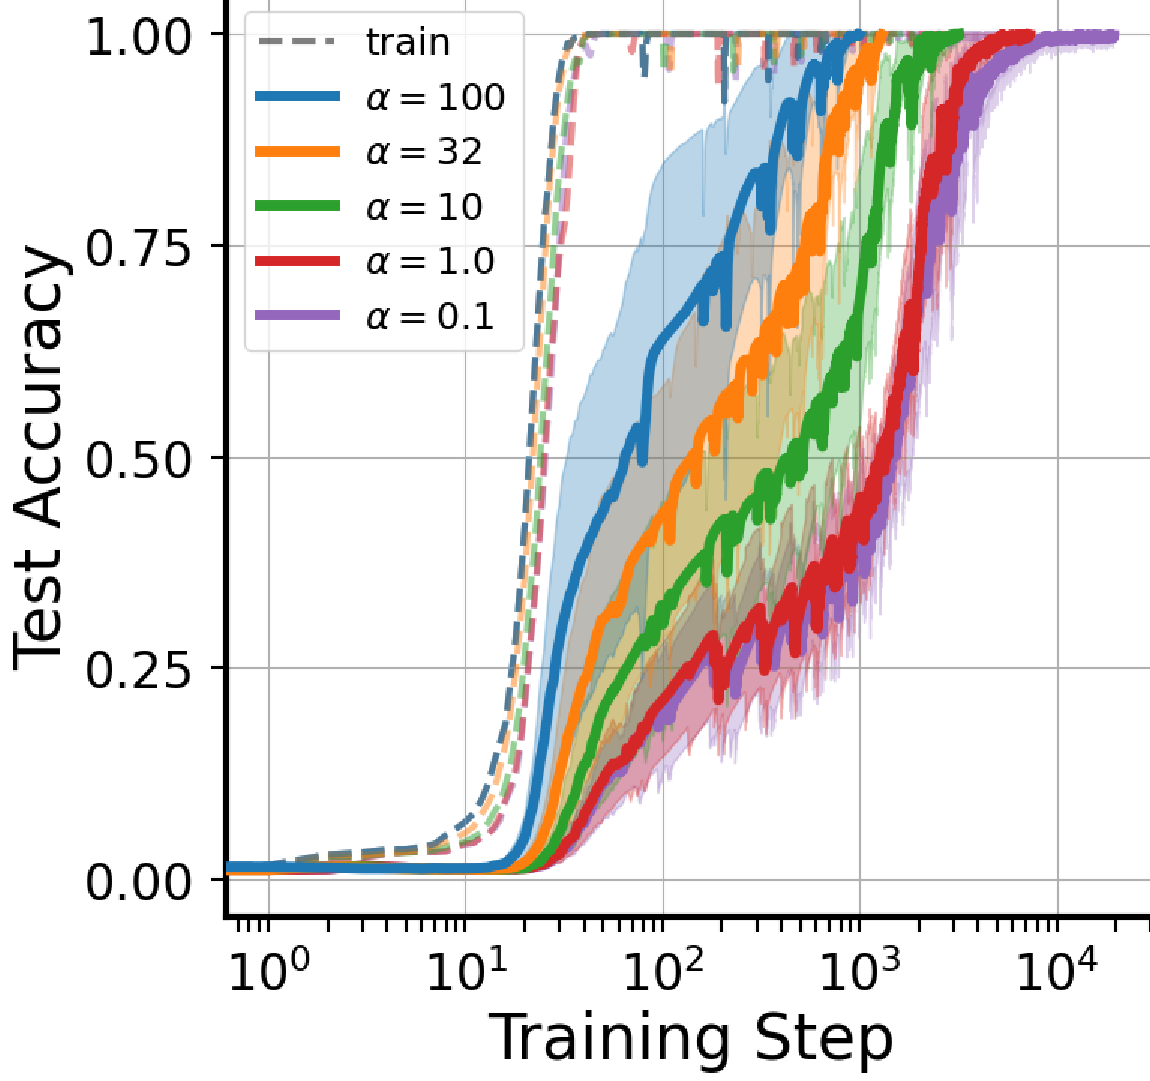
\includegraphics[width=\linewidth]{grokking_iclr_arxiv/figures/grokking.pdf}\vspace{-6mm}
\end{centering}
\caption{Our contributions demonstrated through results obtained in addition modulo 113 task. We show that the delay in generalization induced by NLM can be reversed using the proposed $\perp$\!AdamW ((\textbf{a}) and (\textbf{b})) and that the numerical errors that lead to overfitting instead of grokking can be avoided by using the proposed $\stablemax$ ((\textbf{b}) and (\textbf{c})). \vspace{-5mm}}
\label{fig:teaser}
%\vspace{-3mm}
\end{figure}

\begin{comment}
\begin{figure}[t]
\begin{subfigure}[t]{.32\textwidth}
    \includegraphics[width=\linewidth]{grokking_iclr/figures/teaser_baseline.pdf}
    \caption{AdamW}
\end{subfigure}
\hfill
\begin{subfigure}[t]{.32\textwidth}
    \includegraphics[width=\linewidth]{grokking_iclr/figures/teaser_softermax.pdf}
    \label{fig:input_representations}
    \caption{AdamW + stablemax}
\end{subfigure}%
\hfill
\begin{subfigure}[t]{.32\textwidth}
    \includegraphics[width=\linewidth]{grokking_iclr/figures/teaser_nlm.pdf}
    \label{fig:gradient_norms}
    \caption{$\perp$AdamW + stablemax}
\end{subfigure}
\caption{\vspace{-5mm}}
\vspace{-5mm}
\end{figure}
\end{comment}
\section{Related Work}

%Photorealistic rendering and animation of humans is an important area of research. 
Early works on photorealistic rendering and animation employed traditional computer graphics pipelines which involved large multi-camera setups such as lightstages ~\cite{debevec2012light} to capture the detailed texture and material of the human body. The animation of human bodies involved the rigging of an artist-created template of a human body mesh~\cite{alexander2013digitalira, alexander2010emily}. The introduction of statistical body shape models~\cite{anguelov2005scape, SMPL:2015, pavlakos2019smplx, STAR:ECCV:2020, SUPR} enabled representation of diverse human shape and animation of the human body by a single model. This reduced the manual effort in creating template meshes and rigging them.
%\jg{more quickly? More realistically? more easily? by non professionals?}. 
However, these shape models do not account for many details such as clothing, hair, accessories etc. Follow up works such as DRAPE~\cite{drape2012guan} or CAPE~\cite{ma2020cape} augment the shape models to add an additional layer of clothing or altogether choose a different representation such as occupancy~\cite{saito2019pifu, saito2020pifuhd, chen2021snarf, xiu2023econ, xiu2022icon} to represent the details of the geometry. This led to improved estimation of geometry, however the capturing appearance without large capture setups still remained a challenge.

In recent years, Neural Radiance Fields (NeRF)~\cite{mildenhall2020nerf} have enabled a joint representation of geometry and appearance for view-synthesis using multiview images without the need of a large capture setup. Although, a NeRF is designed for capturing static objects, recent work~\cite{peng2021neuralbody, weng2020vid2actor, liu2021neuralactor, weng2022humannerf, jiang2022neuman, Su21arxiv_A_NeRF, guo2023vid2avatar, Feng2022scarf,Mihajlovic:KeypointNeRF:ECCV2022} has extended the NeRF to enable capturing a dynamic moving humans
%by using a multi-camera setup in a capture lab. 
Weng et al.~\cite{weng2022humannerf} propose a method to model a NeRF representation of a human using a single monocular video enabling 360 degree view generation of a human. Furthermore, NeuMan~\cite{jiang2022neuman} introduces a joint NeRF representation of human and the scene capable of view synthesis and animation of the human in the scene. However, a major limitation of NeRF-based methods is that NeRFs are slow to train and render. Several methods have emerged to speed up training and rendering of NeRFs. These include using an explicit representation such as learning a function at grid points \cite{chen2022tensorf, reiser2021kilonerf}, using hash encoding \cite{muller2022instantngp} or altogether discarding the learnable component~\cite{fridovich2022plenoxels,liu2020neural}. 

Recent work on 3D Gaussian Splatting~\cite{kerbl3Dgaussians} uses a set of 3D Gaussians to represent a scene and renders it by splatting and rasterizing the Gaussians. This approach significantly improves the training and rendering times over traditional NeRFs. Recent work has addressed the extension of 3DGS scenes to controlled dynamic scenes~\cite{wu20234dgs} and multi-camera capture setup~\cite{luiten2023dynamicgs}. However, the 3D Gaussian Splatting framework is not trivial to extend to dynamic humans that allows for both novel-view and novel-pose synthesis of human and the scene.

Our methods builds on the 3D Gaussian Splatting framework~\cite{kerbl3Dgaussians} and utilize the \smpl body shape model~\cite{SMPL:2015} as a prior and learns a deformation model for animation control. 
We use a triplane and three MLPs to coordinate the Gaussians (\eg, their rotation, scale, color, and LBS weights). 
%
%We use a graph representation to bind the Gaussian points and use graph 
% \ar{No graph convs anymore. change this $\rightarrow$}
% convolutions~\cite{graph-conv, coma, cape} to regress the properties of the Gaussian points. 

%While neural fields have established themselves as state-of-the-art approach for representing static 3D scenes, the generalization to dynamic scenes, especially involving humans has been difficult.

%Traditional approaches for representing a human body mainly focused on geometry. Early works~\cite{SMPL:2015, CAPE} learn a mesh representation for humans and their clothing respectively. This enables 
%Following works such as PiFU~\cite{PiFU} use an implicit representation using an occupancy field~\cite{occupancy_nets} .

%GCN works coma, cape, meshcnn
%This problem is inherent to the structure-from-motion ambiguity where the camera motion and the object motion in the scene are entangled. To deal with this, recent approaches~\cite{neuralavatar_zju3d, neuralactor} use multi-camera setup in a capture lab to disentangle camera motion and human motion. 



\subsection{Benchmarking LVLMs on ArXivCap}
\label{subsec:exp_arxivcap}
\subsubsection{Evaluated Tasks}
\label{subsubsec:evaluated_task}
Four vision-to-text tasks to benchmark LVLMs' ability to comprehend scientific figures.
\paragraph{Single-Figure Captioning} 
Similar to the traditional image captioning setup~\citep{lin2014mscoco}, single-figure captioning requires the model to generate a caption for the given single figure. 
The captions generated by the model are expected to encapsulate the nuanced details within these figures, including numbers and mathematical formulas, presenting a unique challenge for models to identify and articulate these elements accurately.
Formally, given an image-caption pair $(I, C)$, the LVLM $\mathcal{M}$ is asked to generate the caption given an instruction prompt $P_s$ to hint the goal of scientific captioning:
\begin{equation*}
    \hat{C} = \mathcal{M} (I, P_s),
\end{equation*}
where $\hat{C}$ would be evaluated according to the ground-truth $C$.
% formalize it 

\paragraph{Multiple-Figure Captioning}
We introduce a more intricate challenge involving applying reasoning across multiple images. This task, termed Multiple-Figure Captioning, necessitates the model to craft a comprehensive summary caption for subfigures. 
As exemplified in Figure~\ref{fig:chunk_example}, the model is tasked with generating an overarching caption for two or more subfigures, leveraging visual clues to draw comparisons and formulate summary captions.
% Specifically, Multiple Image Captioning requires the model to generate a summary caption for a series of related subfigures. For example, as illustrated in \cref{fig:chunk_example}, given two subfigures, the model is asked to generate the overall caption for these two figures by making comparisons and drawing conclusions from the visual clues.
Formally, given a list of figures $L = \left( I_1, \ldots, I_n\right)$, the model is asked to generate the ground-truth main caption $C$ by considering all the semantics in the figures with a task prompt $P_m$:
\begin{equation*}
    \hat{C} = \mathcal{M} ( L, P_m ) = \mathcal{M} ( I_1, \ldots, I_n, P_m).
\end{equation*}


\paragraph{Contextualized Captioning}
Inspired by the evolving in-context learning capabilities of LLMs~\citep{brown2020language,icl_survey}, we introduce a contextualized captioning task to examine the in-context learning ability of LVLMs. 
In this task, the model is presented with a set of figure-caption pairs, and its goal is to generate a caption for a given image based on the provided demonstrations.
Given a sequential image-captions pairs $S = \{ ( I_i, C_i)  \}_{i=1}^n$ consisting of $n$ pairs of image $I_i$ and the corresponding $C_i$, the contextualized image captioning task can be formalized as follows:
\begin{equation*}
    \hat{C_n} = \mathcal{M} ( I_1, C_1, \ldots, I_{n-1}, C_{n-1}, I_n, P_c).
\end{equation*}
The model is supposed to leverage the context history to enhance the accuracy and coherence of the generated caption.

\paragraph{Title Generation}
This task requires a nuanced understanding of figures and captions to distill essential observations into a high-level summary of the presented results for LVLMs.
Specifically, instead of producing the captions for the figures, this task requires the model to connect different figures and corresponding captions to infer the paper title.
Let $S = \{ (I_i, C_i) \}_{i=1}^m$ be a sequence of $m$ figure-caption pairs in the extracted paper. 
Note that $I_i$ could be a single figure or a multiple-figure, and we reuse $I_i$ for simplicity here.
The title generation asks $\mathcal{M}$ to generate the title for the paper given a task prompt $P_t$:
\begin{equation*}
   \hat{T} = \mathcal{M} ( I_1, C_1, \ldots, I_{m}, C_m, P_t ) .
\end{equation*}
The prediction $\hat{T}$ is evaluated by comparing it to the original title $T$.





\begin{figure*}[t]
    \centering
    \includegraphics[width=\linewidth]{figures/pdf_files/sota_qual.pdf}
    \small
    \begin{tabular}{cccc}
         \quad Ground Truth \qquad \qquad & \qquad \qquad HUGS (ours) \qquad \qquad & \qquad \quad \qquad NeuMan~\cite{jiang2022neuman} \qquad \quad & \qquad \quad \qquad Vid2Avatar~\cite{guo2023vid2avatar} \qquad 
    \end{tabular}
    \vspace{-3mm}
    \caption{Qualitative results comparing HUGS (ours) with NeuMan and Vid2Avatar with full human (left) and zoomed-in regions (right) for each of the methods. HUGS shows better reconstruction quality especially around hands, feet and clothing wrinkles.} 
    \label{fig:qualitative_sota}
\end{figure*}{}
\begin{figure*}
    \centering
    \includegraphics[width=\linewidth]{figures/pdf_files/novel_pose_scene.pdf}
    \caption{Rendering obtained by transferring the Human Gaussians to a different scene. Top-left corner shows the original scene in which the human was captured.}
    \label{fig:composition}
\end{figure*}{}

\section{Experiments}
% \subsection{Implementation details}
\subsection{Datasets}
% \paragraph{NeuMan} We use NeuMan dataset, a collection of 6 videos about 10 to 20 seconds long each, with a single person captured using a mobile phone. Moreover, the camera reasonably pans through the scene to enable multi-view reconstruction. The sequences are named – Seattle, Citron, Parking, Bike, Jogging and Lab. Following the ~\cite{jiang2022neuman} we split frames into 80\% training frames, 10\% validation frames, and 10\% test frames.

% \paragraph{ZJU-MoCap} We evaluate our method on the ZJU-MoCap dataset~\cite{zjumocap} For ZJU-MoCap, following \cite{weng2022humannerf} we select 6 subjects (377, 386, 387, 392, 393, 394) with diverse motions and use images captured by "camera 1" as input and the other 22 cameras for evaluation. We directly apply camera matrices, body pose, and segmentation provided by the dataset.
\paragraph{NeuMan Dataset~\cite{jiang2022neuman}} consists of six videos, each lasting between 10 to 20 seconds, featuring a single individual captured using a mobile phone. The camera pans through the scenes, facilitating multi-view reconstruction. The sequences are denoted as Seattle, Citron, Parking, Bike, Jogging, and Lab. Following the approach outlined in~\cite{jiang2022neuman}, we split frames into 80\% training frames, 10\% validation frames, and 10\% test frames.

\paragraph{ZJU-MoCap Dataset~\cite{peng2021neuralbody}} consists of videos of a human captured in a lab using multi-view capture setup. To align with the methodology in~\cite{weng2022humannerf,yu2023monohuman}, we select six subjects (377, 386, 387, 392, 393, 394) showcasing diverse motions. We employed images captured by "camera 1" as input and utilized the other 22 cameras for evaluation. The camera matrices, body pose, and segmentation provided by the dataset were directly applied in our evaluation process.

\subsection{Qualitative Results}
\label{sec:qualitative}
\paragraph{State-of-the-art Comparison.} We show the qualitative results of our method in ~\cref{fig:qualitative_sota} and compare it with Vid2Avatar~\cite{guo2023vid2avatar} and NeuMan~\cite{jiang2022neuman}. The results are shown from the test samples of the NeuMan dataset~\cite{jiang2022neuman} that are not seen during training.
In the scene background regions, HUGS shows better reconstruction quality than both Vid2Avatar and NeuMan. Vid2Avatar shows blurry scene reconstruction with several artifacts. In contrast, NeuMan shows better scene reconstruction quality but misses fine details such as the house numbers (zoomed-in) in the first row, the wooden plank (zoomed-in) in the second row and the cupboard (zoomed-in) in the third row. In comparison, HUGS shows better reconstruction quality and preserves these fine details as shown in the zoomed-in regions.

In the human regions, Vid2Avatar shows artifacts in the hand region (row 1) and blurry reconstruction in the feet (row 2) and arm region (row 3). In contrast, NeuMan gets better details of the feet regions in some cases (row 2) and introduces artifacts in hands (row 2) and feet (row 3) regions in other cases. In comparison, our method preserves the details around hand and feet and shows better reconstruction quality. Furthermore, our method also preserves the structure around clothing (row 1) where the wrinkles are reconstructed well while preserving the structure of the zipper (zoomed-in) around it compared to previous work.

In summary, we note that HUGS shows better reconstruction quality of both the scene and the human as compared to previous methods while being orders of magnitude faster to train and render (see \S \ref{sec:timing} for speed comparison). We will provide additional qualitative results with videos in the Supp. Mat.

\begin{figure}[t]
    \centering
    \includegraphics[width=\linewidth]{figures/pdf_files/neuman_canonical.pdf}
    \begin{tabular}{cc}
         NeuMan~\cite{jiang2022neuman} \quad \quad & \qquad \qquad HUGS (ours) 
    \end{tabular}
    \caption{Visualization of Human in canonical Da-pose for HUGS (ours) showing qualitative improvements over NeuMan~\cite{jiang2022neuman}.} 
    \label{fig:canonical}
\end{figure}
\paragraph{Canonical Human Shapes.} In ~\cref{fig:canonical}, we show the reconstruction of the human in the canonical space. We note that our method captures fine details around the feet and hands of the human which look noisy in the case of NeuMan~\cite{jiang2022neuman}. Furthermore, we note that our method preserves rich details on the face. This enables us to achieve high reconstruction quality during the animation phase. 

\definecolor{tabfirst}{rgb}{1, 0.7, 0.7}
\definecolor{tabsecond}{rgb}{1, 0.85, 0.7}
\definecolor{tabthird}{rgb}{1, 1, 0.7}

\begin{table*}[]
    \centering
    \resizebox{\textwidth}{!}{
    \begin{tabular}{c|ccc|ccc|ccc|ccc|ccc|ccc}
    \toprule
        & \multicolumn{3}{c|}{\textbf{Seattle}} & \multicolumn{3}{c|}{\textbf{Citron}} & \multicolumn{3}{c|}{\textbf{Parking}} & \multicolumn{3}{c|}{\textbf{Bike}} & \multicolumn{3}{c|}{\textbf{Jogging}} & \multicolumn{3}{c}{\textbf{Lab}}   \\
    \midrule
        & PSNR $\uparrow$ & SSIM $\uparrow$ & LPIPS $\downarrow$ & PSNR $\uparrow$ & SSIM $\uparrow$ & LPIPS $\downarrow$ & PSNR $\uparrow$ & SSIM $\uparrow$ & LPIPS $\downarrow$ & PSNR $\uparrow$ & SSIM $\uparrow$ & LPIPS $\downarrow$ & PSNR $\uparrow$ & SSIM $\uparrow$ & LPIPS $\downarrow$ & PSNR $\uparrow$ & SSIM $\uparrow$ & LPIPS $\downarrow$  \\
    \midrule
    NeRF-T &        21.84       &      0.69              &       0.37           &               12.33  &          0.49            &        0.65             &       21.98            &             0.69        &        0.46    &   21.16     &      0.71         &     0.36         &     20.63        &       0.53         &         0.49        &     20.52         &    0.75      &       0.39                \\
    % \midrule
    HyperNeRF &    16.43            &     0.43         &    0.40            &     16.81            &    0.41        &          0.56        &      16.04           &           0.38      &         0.62    &     17.64     &   0.42   &      0.43  &       18.52          &  0.39    & 0.52               &      16.75      &    0.51      &     0.23       \\

    
    % \midrule
    Vid2Avatar &  \cellcolor{tabthird}17.41 &  \cellcolor{tabthird}0.56 &  \cellcolor{tabthird}0.60 &  \cellcolor{tabthird}14.32 &  \cellcolor{tabthird}0.62 &  \cellcolor{tabthird}0.65 &  \cellcolor{tabthird}21.56 &  \cellcolor{tabthird}0.69 &  \cellcolor{tabthird}0.50 &  \cellcolor{tabthird}14.86 &  \cellcolor{tabthird}0.51 &  \cellcolor{tabthird}0.69 &  \cellcolor{tabthird}15.04 &  \cellcolor{tabthird}0.41 &  \cellcolor{tabthird}0.70 &  \cellcolor{tabthird}13.96 &  \cellcolor{tabthird}0.60 &  \cellcolor{tabthird}0.68 \\
    % \midrule
    NeuMan     & \cellcolor{tabsecond}23.99 & \cellcolor{tabsecond}0.78 & \cellcolor{tabsecond}0.26 & \cellcolor{tabsecond}24.63 & \cellcolor{tabsecond}0.81 & \cellcolor{tabsecond}0.26 & \cellcolor{tabsecond}25.43 & \cellcolor{tabsecond}0.80 & \cellcolor{tabsecond}0.31 &  \cellcolor{tabfirst}25.55 & \cellcolor{tabsecond}0.83 & \cellcolor{tabsecond}0.23 & \cellcolor{tabsecond}22.70 & \cellcolor{tabsecond}0.68 & \cellcolor{tabsecond}0.32 & \cellcolor{tabsecond}24.96 & \cellcolor{tabsecond}0.86 & \cellcolor{tabsecond}0.21 \\
    \midrule
    HUGS       &  \cellcolor{tabfirst}25.94 &  \cellcolor{tabfirst}0.85 &  \cellcolor{tabfirst}0.13 &  \cellcolor{tabfirst}25.54 &  \cellcolor{tabfirst}0.86 &  \cellcolor{tabfirst}0.15 &  \cellcolor{tabfirst}26.86 &  \cellcolor{tabfirst}0.85 &  \cellcolor{tabfirst}0.22 & \cellcolor{tabsecond}25.46 &  \cellcolor{tabfirst}0.84 &  \cellcolor{tabfirst}0.13 &  \cellcolor{tabfirst}23.75 &  \cellcolor{tabfirst}0.78 &  \cellcolor{tabfirst}0.22 &  \cellcolor{tabfirst}26.00 &  \cellcolor{tabfirst}0.92 &  \cellcolor{tabfirst}0.09
    \\
    \bottomrule
    \end{tabular}  
    }
    \caption{Comparison of HUGS (ours) with previous work on test images of the NeuMan dataset~\cite{jiang2022neuman} using PSNR, SSIM and LPIPS metrics. HUGS achieves state-of-the-art performance across every category with the exception of PSNR on the \textit{Bike} sequence.}
    \label{tab:neuman_human_scene}
\end{table*}
\definecolor{tabfirst}{rgb}{1, 0.7, 0.7}
\definecolor{tabsecond}{rgb}{1, 0.85, 0.7}
\definecolor{tabthird}{rgb}{1, 1, 0.7}

\begin{table*}[htb!]
    \centering
    \resizebox{\textwidth}{!}{
    \begin{tabular}{c|ccc|ccc|ccc|ccc|ccc|ccc}
    \toprule
        & \multicolumn{3}{c|}{\textbf{Seattle}} & \multicolumn{3}{c|}{\textbf{Citron}} & \multicolumn{3}{c|}{\textbf{Parking}} & \multicolumn{3}{c|}{\textbf{Bike}} & \multicolumn{3}{c|}{\textbf{Jogging}} & \multicolumn{3}{c}{\textbf{Lab}}   \\
    \midrule
        & PSNR $\uparrow$ & SSIM $\uparrow$ & LPIPS $\downarrow$ & PSNR $\uparrow$ & SSIM $\uparrow$ & LPIPS $\downarrow$ & PSNR $\uparrow$ & SSIM $\uparrow$ & LPIPS $\downarrow$ & PSNR $\uparrow$ & SSIM $\uparrow$ & LPIPS $\downarrow$ & PSNR $\uparrow$ & SSIM $\uparrow$ & LPIPS $\downarrow$ & PSNR $\uparrow$ & SSIM $\uparrow$ & LPIPS $\downarrow$ \\
    \midrule 
    Vid2Avatar &  \cellcolor{tabthird}16.90 &  \cellcolor{tabthird}0.51 &  \cellcolor{tabthird}0.27 &  \cellcolor{tabthird}15.96 &  \cellcolor{tabthird}0.59 &  \cellcolor{tabthird}0.28 & \cellcolor{tabsecond}18.51 &  \cellcolor{tabthird}0.65 &  \cellcolor{tabthird}0.26 &  \cellcolor{tabthird}12.44 &  \cellcolor{tabthird}0.39 &  \cellcolor{tabthird}0.54 &  \cellcolor{tabthird}16.36 &  \cellcolor{tabthird}0.46 &  \cellcolor{tabthird}0.30 &  \cellcolor{tabthird}15.99 &  \cellcolor{tabthird}0.62 &  \cellcolor{tabthird}0.34 \\
    % \midrule
    NeuMan     & \cellcolor{tabsecond}18.42 & \cellcolor{tabsecond}0.58 & \cellcolor{tabsecond}0.20 & \cellcolor{tabsecond}18.39 & \cellcolor{tabsecond}0.64 & \cellcolor{tabsecond}0.19 &  \cellcolor{tabthird}17.66 & \cellcolor{tabsecond}0.66 & \cellcolor{tabsecond}0.24 & \cellcolor{tabsecond}19.05 & \cellcolor{tabsecond}0.66 & \cellcolor{tabsecond}0.21 &  \cellcolor{tabfirst}17.57 & \cellcolor{tabsecond}0.54 & \cellcolor{tabsecond}0.29 & \cellcolor{tabsecond}18.76 & \cellcolor{tabsecond}0.73 & \cellcolor{tabsecond}0.23 \\
    \midrule
    HUGS       &  \cellcolor{tabfirst}19.06 &  \cellcolor{tabfirst}0.67 &  \cellcolor{tabfirst}0.15 &  \cellcolor{tabfirst}19.16 &  \cellcolor{tabfirst}0.71 &  \cellcolor{tabfirst}0.16 &  \cellcolor{tabfirst}19.44 &  \cellcolor{tabfirst}0.73 &  \cellcolor{tabfirst}0.17 &  \cellcolor{tabfirst}19.48 &  \cellcolor{tabfirst}0.67 &  \cellcolor{tabfirst}0.18 & \cellcolor{tabsecond}17.45 &  \cellcolor{tabfirst}0.59 &  \cellcolor{tabfirst}0.27 &  \cellcolor{tabfirst}18.79 &  \cellcolor{tabfirst}0.76 &  \cellcolor{tabfirst}0.18
    
\\
    \bottomrule
    \end{tabular}  
    }
    \caption{Comparison of HUGS (ours) with previous work on the NeuMan dataset~\cite{jiang2022neuman} over \textbf{human-only} regions cropped using a tight bounding box. Performance is evaluated on PSNR, SSIM and LPIPS metrics.}
    \label{tab:neuman_human}
\end{table*}
\definecolor{tabfirst}{rgb}{1, 0.7, 0.7}
\definecolor{tabsecond}{rgb}{1, 0.85, 0.7}
\definecolor{tabthird}{rgb}{1, 1, 0.7}

\begin{table*}[htb!]
    \centering
    \resizebox{\textwidth}{!}{
    \begin{tabular}{c|ccc|ccc|ccc|ccc|ccc|ccc}
    \toprule
        & \multicolumn{3}{c|}{\textbf{377}} & \multicolumn{3}{c|}{\textbf{386}} & \multicolumn{3}{c|}{\textbf{387}} & \multicolumn{3}{c|}{\textbf{392}} & \multicolumn{3}{c|}{\textbf{393}} & \multicolumn{3}{c}{\textbf{394}}   \\
    \midrule
        & PSNR $\uparrow$ & SSIM $\uparrow$ & LPIPS $\downarrow$ & PSNR $\uparrow$ & SSIM $\uparrow$ & LPIPS $\downarrow$ & PSNR $\uparrow$ & SSIM $\uparrow$ & LPIPS $\downarrow$ & PSNR $\uparrow$ & SSIM $\uparrow$ & LPIPS $\downarrow$ & PSNR $\uparrow$ & SSIM $\uparrow$ & LPIPS $\downarrow$ & PSNR $\uparrow$ & SSIM $\uparrow$ & LPIPS $\downarrow$  \\
    \midrule
    %     NeuralBody & 29.11 & 0.97 & 40.95 & 30.54 & 0.97 & 46.43 & 27.00 & 0.95 & 59.47 & 30.10 & 0.96 & 53.27 & 28.61 & 0.96 & 59.05 & 29.10 & 0.96 & 54.55 & 1 days \\
    % \midrule
    %     HumanNerf & 30.41 & 0.97 & 24.06 & 33.20 & 0.98 & 28.99 & 28.18 & 0.96 & 35.58 & 31.04 & 0.97 & 32.12 & 28.31 & 0.96 & 36.72 & 30.31 & 0.96 & \textbf{32.89} & 1 days \\
    % \midrule
    %     MonoHuman & 30.77 & 0.98 & \textbf{21.67} & 32.97 & 0.97 & 32.73 & 27.93 & 0.96 & \textbf{33.45} & 31.24 & 0.97 & \textbf{31.04} & 28.46 & 0.96 & 34.24 & 28.94 & 0.96 & 35.90 & 1 days \\
    % \midrule
    %     HUGS      & \textbf{30.89} & \textbf{0.98} & 26.13 & \textbf{34.00 }& \textbf{0.98} & \textbf{28.78} &\textbf{ 29.41} & \textbf{0.97} & 35.04 & \textbf{31.75} & \textbf{0.98} & 31.32 & \textbf{29.91} & \textbf{0.97} & \textbf{34.70} & \textbf{31.06} & \textbf{ 0.97} & 33.13 & 35 mins \\ 

NeuralBody &                      29.11 & \cellcolor{tabsecond}0.97 & \cellcolor{tabsecond}0.04 &                      30.54 & \cellcolor{tabsecond}0.97 &  \cellcolor{tabthird}0.05 &                      27.00 &  \cellcolor{tabthird}0.95 &  \cellcolor{tabthird}0.06 &                      30.10 & \cellcolor{tabsecond}0.96 & \cellcolor{tabsecond}0.05 & \cellcolor{tabsecond}28.61 & \cellcolor{tabsecond}0.96 &  \cellcolor{tabthird}0.06 &  \cellcolor{tabthird}29.10 & \cellcolor{tabsecond}0.96 &  \cellcolor{tabthird}0.05 \\

HumanNerf  &  \cellcolor{tabthird}30.41 & \cellcolor{tabsecond}0.97 &  \cellcolor{tabfirst}0.02 & \cellcolor{tabsecond}33.20 &  \cellcolor{tabfirst}0.98 & \cellcolor{tabsecond}0.03 & \cellcolor{tabsecond}28.18 & \cellcolor{tabsecond}0.96 & \cellcolor{tabsecond}0.04 &  \cellcolor{tabthird}31.04 &  \cellcolor{tabfirst}0.97 &  \cellcolor{tabfirst}0.03 &                      28.31 & \cellcolor{tabsecond}0.96 & \cellcolor{tabsecond}0.04 & \cellcolor{tabsecond}30.31 & \cellcolor{tabsecond}0.96 &  \cellcolor{tabfirst}0.03  \\
MonoHuman  & \cellcolor{tabsecond}30.77 &  \cellcolor{tabfirst}0.98 &  \cellcolor{tabfirst}0.02 &  \cellcolor{tabthird}32.97 & \cellcolor{tabsecond}0.97 & \cellcolor{tabsecond}0.03 &  \cellcolor{tabthird}27.93 & \cellcolor{tabsecond}0.96 &  \cellcolor{tabfirst}0.03 & \cellcolor{tabsecond}31.24 &  \cellcolor{tabfirst}0.97 &  \cellcolor{tabfirst}0.03 &  \cellcolor{tabthird}28.46 & \cellcolor{tabsecond}0.96 &  \cellcolor{tabfirst}0.03 &                      28.94 & \cellcolor{tabsecond}0.96 & \cellcolor{tabsecond}0.04  \\
\midrule
\acronym   &  \cellcolor{tabfirst}30.80 &  \cellcolor{tabfirst}0.98 &  \cellcolor{tabfirst}0.02 &  \cellcolor{tabfirst}34.11 &  \cellcolor{tabfirst}0.98 &  \cellcolor{tabfirst}0.02 &  \cellcolor{tabfirst}29.29 &  \cellcolor{tabfirst}0.97 &  \cellcolor{tabfirst}0.03 &  \cellcolor{tabfirst}31.36 &  \cellcolor{tabfirst}0.97 &  \cellcolor{tabfirst}0.03 &  \cellcolor{tabfirst}29.80 &  \cellcolor{tabfirst}0.97 &  \cellcolor{tabfirst}0.03 &  \cellcolor{tabfirst}30.54 &  \cellcolor{tabfirst}0.97 &  \cellcolor{tabfirst}0.03  \\

    \bottomrule
    \end{tabular}  
    }
    \caption{Comparison of HUGS (ours) with the previous work on the ZJU Mocap dataset~\cite{peng2021neuralbody}. Performance is evaluated on PSNR, SSIM and LPIPS metric. HUGS achieves state-of-the-art performance across all scenes and all metrics.}
    \label{tab:zju}
\end{table*}



\paragraph{Disentanglement of the Human and the Scene.} HUGS allows for a disentangled represenation of the human and the scene by storing their Gaussian features separately. This allows us to move the human to different scenes. In \cref{fig:composition}, we show the composition of human captured in one scene into a different scene. We show additional video results in the supplemental material.


\subsection{Quantitative Results}
\label{sec:quantitative}
We compare the performance of our method with baselines such as NeRF-T~\cite{li2021neural}, HyperNeRF~\cite{park2021hypernerf} and the existing state-of-the-art methods -- NeuMan~\cite{jiang2022neuman} and Vid2Avatar~\cite{guo2023vid2avatar}.

In \cref{tab:neuman_human_scene}, we evaluate the reconstruction quality on the NeuMan dataset~\cite{jiang2022neuman} on three different metrics -- Peak Signal-to-Noise Ration (PSNR), SSIM~\cite{ssim} and LPIPS~\cite{zhang2018lpips}. NeRF-T and HyperNeRF are general dynamic scene reconstruction methods and do not specialize for humans. Therefore, they show poor reconstruction quality. On the other hand, NeuMan and Vid2Avatar employ specialized models for the human and the scene. NeuMan employs a NeRF-based~\cite{mildenhall2020nerf} approach for both scene and human modeling. Vid2Avatar utilizes an implicit SDF model and volume rendering for scene and human representation. Therefore, both NeuMan and Vid2Avatar show improved reconstruction quality. In comparison, our method achieves state-of-the-art performance across all the scenes and metrics except PSNR on the \textit{Bike} sequence where we show competitive performance.

In \cref{tab:neuman_human}, we further evaluate the reconstruction error but only on the regions containing the human. We first take a tight crop around the human region in the ground truth image. This crop is used over all the predictions, and the reconstruction error is evaluated over the cropped samples. It should be noted that we take rectangular crops of the region and do not use any segmentation mask since reconstruction metrics are highly sensitive to masks. Under this evaluation, we show state-of-the-art performance across all scenes and metrics except PSNR on the \textit{Jogging} sequence where we show competitive performance. 

In addition, we evaluate our method using the ZJU Mocap dataset~\cite{peng2021neuralbody} in ~\cref{tab:zju}. We compare with recent previous work that report their evaluation on this dataset which include NeuralBody~\cite{peng2021neuralbody}, HumanNerf~\cite{weng2022humannerf}, and MonoHuman~\cite{yu2023monohuman}. 

%As these models are all NeRF-based, they share the drawback of being slow in both training and rendering. Notably, our method stands out as both faster and more accurate than the listed state-of-the-art models, providing a compelling combination of efficiency and precision.



%In \cref{tab:neuman_human_scene} \cref{tab:neuman_human}, we present a comparative analysis of our method against existing joint human and scene novel view synthesis approaches. Given the novelty of this task, research in this domain is limited. Notable existing works include NeuMan~\cite{jiang2022neuman} and Vid2Avatar~\cite{guo2023vid2avatar}.

\label{sec:timing}
\begin{figure}[t]
    \centering
    \includegraphics[width=0.49\linewidth]{figures/pngs/train_time.png}
    \includegraphics[width=0.49\linewidth]{figures/pngs/render_time.png}
    \caption{{Timing comparison for training in hours and rendering in milliseconds. y-axis is  on log-scale. HUGS outperforms previous methods by an order of magnitude. }} 
    \label{fig:timing}
\end{figure}
\begin{table*}[t]
    \centering
    \resizebox{\textwidth}{!}{
    \begin{tabular}{l|ccc|ccc|ccc|ccc|ccc|ccc}
    \toprule
        & \multicolumn{3}{c|}{\textbf{Seattle}} & \multicolumn{3}{c|}{\textbf{Citron}} & \multicolumn{3}{c|}{\textbf{Parking}} & \multicolumn{3}{c|}{\textbf{Bike}} & \multicolumn{3}{c|}{\textbf{Jogging}} & \multicolumn{3}{c}{\textbf{Lab}}   \\
    \midrule
        & PSNR $\uparrow$ & SSIM $\uparrow$ & LPIPS $\downarrow$ & PSNR $\uparrow$ & SSIM $\uparrow$ & LPIPS $\downarrow$ & PSNR $\uparrow$ & SSIM $\uparrow$ & LPIPS $\downarrow$ & PSNR $\uparrow$ & SSIM $\uparrow$ & LPIPS $\downarrow$ & PSNR $\uparrow$ & SSIM $\uparrow$ & LPIPS $\downarrow$ & PSNR $\uparrow$ & SSIM $\uparrow$ & LPIPS $\downarrow$  \\
    \midrule
    w/o LBS             &                      18.47 & \cellcolor{tabsecond}0.66 & \cellcolor{tabsecond}0.16 & \cellcolor{tabsecond}19.00 & \cellcolor{tabsecond}0.70 &  \cellcolor{tabfirst}0.16 & \cellcolor{tabsecond}19.13 & \cellcolor{tabsecond}0.72 & \cellcolor{tabsecond}0.19 & \cellcolor{tabsecond}19.73 &  \cellcolor{tabfirst}0.68 &  \cellcolor{tabfirst}0.18 &                      17.29 &  \cellcolor{tabthird}0.58 &  \cellcolor{tabthird}0.27 &  \cellcolor{tabthird}18.80 &  \cellcolor{tabfirst}0.76 &  \cellcolor{tabfirst}0.18 \\
    \midrule
    w/o Densify         & \cellcolor{tabsecond}18.91 &  \cellcolor{tabthird}0.65 & \cellcolor{tabsecond}0.16 &                      17.18 &  \cellcolor{tabthird}0.68 &  \cellcolor{tabthird}0.18 &  \cellcolor{tabthird}19.00 &  \cellcolor{tabthird}0.71 &  \cellcolor{tabthird}0.21 &  \cellcolor{tabfirst}19.92 & \cellcolor{tabsecond}0.67 & \cellcolor{tabsecond}0.19 & \cellcolor{tabsecond}17.63 &                      0.57 & \cellcolor{tabsecond}0.26 &  \cellcolor{tabfirst}18.98 &  \cellcolor{tabfirst}0.76 &  \cellcolor{tabfirst}0.18 \\
    \midrule
    w/o $\mathcal{L}^h$ &  \cellcolor{tabthird}18.87 &  \cellcolor{tabfirst}0.67 & \cellcolor{tabsecond}0.16 &  \cellcolor{tabthird}17.31 &                      0.67 &                      0.19 &                      17.76 &                      0.70 &                      0.23 &  \cellcolor{tabthird}19.63 &  \cellcolor{tabfirst}0.68 & \cellcolor{tabsecond}0.19 &  \cellcolor{tabfirst}18.23 &  \cellcolor{tabfirst}0.60 & \cellcolor{tabsecond}0.26 &                      18.75 &  \cellcolor{tabfirst}0.76 & \cellcolor{tabsecond}0.19 \\
    \midrule
    w/o Triplane        &                      18.70 &  \cellcolor{tabthird}0.65 &  \cellcolor{tabfirst}0.15 &                      17.12 &                      0.67 & \cellcolor{tabsecond}0.17 &                      18.78 &                      0.69 & \cellcolor{tabsecond}0.19 &                      19.52 &  \cellcolor{tabthird}0.66 &  \cellcolor{tabfirst}0.18 &  \cellcolor{tabthird}17.60 &                      0.56 &  \cellcolor{tabfirst}0.25 & \cellcolor{tabsecond}18.91 & \cellcolor{tabsecond}0.74 & \cellcolor{tabsecond}0.19 \\
    \midrule
    HUGS                &  \cellcolor{tabfirst}19.06 &  \cellcolor{tabfirst}0.67 &  \cellcolor{tabfirst}0.15 &  \cellcolor{tabfirst}19.16 &  \cellcolor{tabfirst}0.71 &  \cellcolor{tabfirst}0.16 &  \cellcolor{tabfirst}19.44 &  \cellcolor{tabfirst}0.73 &  \cellcolor{tabfirst}0.17 &                      19.48 & \cellcolor{tabsecond}0.67 &  \cellcolor{tabfirst}0.18 &                      17.45 & \cellcolor{tabsecond}0.59 &  \cellcolor{tabthird}0.27 &                      18.79 &  \cellcolor{tabfirst}0.76 &  \cellcolor{tabfirst}0.18
    \\ 
    \bottomrule
    \end{tabular}  
    }
    \caption{\textbf{Ablation study.} The performance is evaluated over human-only bounding box regions using PSNR, SSIM and LPIPS metrics. }
    \label{tab:neuman_ablation_human_only}
\end{table*}

\paragraph{Speed.} In ~\cref{fig:timing}, we compare the training and rendering time of our method with previous work. The use of 3DGS~\cite{kerbl3Dgaussians} speeds up our training and rendering times by a significant margin. We note that HUGS is {$96 \times$} faster than Vid2Avatar and {$336 \times $} faster than NeuMan  training within 30 minutes.
At rendering time, we do not rely on MLPs and only use the LBS weights, enabling higher frame rate.
%
Our method achieves {60 FPS} outperforming NeuMan by {${\sim}7600 \times$} and Vid2Avatar by {${\sim}3800 \times$}. We benchmark all the methods on a single GeForce 3090Ti GPU. \\
%Furthermore, our method enables training within 30 minutes \ar{z times} faster than NeuMan.

%However, NeRF models are characterized by lengthy training and rendering times. Vid2Avatar, on the other hand, utilizes an implicit SDF model and volume rendering for scene and human representation, but this method proves to be prohibitively slow, as indicated by the training and inference time comparison in the tables. In contrast, 

In summary, our model demonstrates efficiency in both training and rendering, delivering superior results compared to existing methods. 
Our model not only outperforms established NeRF and implicit-SDF based models but does so at orders of magnitude faster speeds.


\subsection{Ablation Experiments}
% \begin{table*}[]
    \centering
    \resizebox{\textwidth}{!}{
    \begin{tabular}{l|ccc|ccc|ccc|ccc|ccc|ccc}
    \toprule
        & \multicolumn{3}{c|}{\textbf{Seattle}} & \multicolumn{3}{c|}{\textbf{Citron}} & \multicolumn{3}{c|}{\textbf{Parking}} & \multicolumn{3}{c|}{\textbf{Bike}} & \multicolumn{3}{c|}{\textbf{Jogging}} & \multicolumn{3}{c}{\textbf{Lab}}   \\
    \midrule
        & PSNR $\uparrow$ & SSIM $\uparrow$ & LPIPS $\downarrow$ & PSNR $\uparrow$ & SSIM $\uparrow$ & LPIPS $\downarrow$ & PSNR $\uparrow$ & SSIM $\uparrow$ & LPIPS $\downarrow$ & PSNR $\uparrow$ & SSIM $\uparrow$ & LPIPS $\downarrow$ & PSNR $\uparrow$ & SSIM $\uparrow$ & LPIPS $\downarrow$ & PSNR $\uparrow$ & SSIM $\uparrow$ & LPIPS $\downarrow$  \\
    \midrule
    w/o LBS             &                      25.80 &  \cellcolor{tabfirst}0.85 & \cellcolor{tabsecond}0.14 & \cellcolor{tabsecond}25.36 &  \cellcolor{tabfirst}0.86 &  \cellcolor{tabfirst}0.15 & \cellcolor{tabsecond}26.68 &  \cellcolor{tabfirst}0.85 & \cellcolor{tabsecond}0.23 &  \cellcolor{tabfirst}25.62 & \cellcolor{tabsecond}0.84 &  \cellcolor{tabfirst}0.13 &  \cellcolor{tabthird}23.70 &  \cellcolor{tabfirst}0.78 & \cellcolor{tabsecond}0.22 & \cellcolor{tabsecond}25.96 & \cellcolor{tabsecond}0.91 &  \cellcolor{tabfirst}0.09 \\
    \midrule
    w/o Densify         &                      25.52 &  \cellcolor{tabthird}0.83 &                      0.17 &                      21.65 & \cellcolor{tabsecond}0.83 & \cellcolor{tabsecond}0.19 &                      24.32 &  \cellcolor{tabthird}0.80 &                      0.31 & \cellcolor{tabsecond}25.61 &  \cellcolor{tabthird}0.83 &  \cellcolor{tabthird}0.16 &                      21.37 &  \cellcolor{tabthird}0.73 &                      0.26 &                      23.95 &  \cellcolor{tabthird}0.90 &  \cellcolor{tabthird}0.11 \\
    \midrule
    w/o $\mathcal{L}^h$ &  \cellcolor{tabfirst}26.34 &  \cellcolor{tabfirst}0.85 &  \cellcolor{tabfirst}0.13 &  \cellcolor{tabthird}24.60 &  \cellcolor{tabfirst}0.86 &  \cellcolor{tabfirst}0.15 &  \cellcolor{tabthird}25.48 &  \cellcolor{tabfirst}0.85 &  \cellcolor{tabthird}0.25 &  \cellcolor{tabfirst}25.62 &  \cellcolor{tabfirst}0.85 &  \cellcolor{tabfirst}0.13 &  \cellcolor{tabfirst}24.10 &  \cellcolor{tabfirst}0.78 &  \cellcolor{tabfirst}0.21 &  \cellcolor{tabthird}25.94 & \cellcolor{tabsecond}0.91 & \cellcolor{tabsecond}0.10 \\
    \midrule
    w/o Triplane        & \cellcolor{tabsecond}25.96 & \cellcolor{tabsecond}0.84 &  \cellcolor{tabthird}0.15 &                      21.93 & \cellcolor{tabsecond}0.83 & \cellcolor{tabsecond}0.19 &                      23.90 & \cellcolor{tabsecond}0.81 &                      0.30 &  \cellcolor{tabthird}25.49 & \cellcolor{tabsecond}0.84 & \cellcolor{tabsecond}0.15 &                      22.02 & \cellcolor{tabsecond}0.74 &  \cellcolor{tabthird}0.25 &                      22.65 &                      0.89 &                      0.12 \\
    \midrule
    HUGS                &  \cellcolor{tabthird}25.94 &  \cellcolor{tabfirst}0.85 &  \cellcolor{tabfirst}0.13 &  \cellcolor{tabfirst}25.54 &  \cellcolor{tabfirst}0.86 &  \cellcolor{tabfirst}0.15 &  \cellcolor{tabfirst}26.86 &  \cellcolor{tabfirst}0.85 &  \cellcolor{tabfirst}0.22 &                      25.46 & \cellcolor{tabsecond}0.84 &  \cellcolor{tabfirst}0.13 & \cellcolor{tabsecond}23.75 &  \cellcolor{tabfirst}0.78 & \cellcolor{tabsecond}0.22 &  \cellcolor{tabfirst}26.00 &  \cellcolor{tabfirst}0.92 &  \cellcolor{tabfirst}0.09
    \\ 
    \bottomrule
    \end{tabular}  
    }
    \caption{NeuMan Ablation experiments}
    \label{tab:neuman_ablation}
\end{table*}
\begin{figure}[t]
    \centering
    \includegraphics[width=\linewidth]{figures/pdf_files/ablation_qual.pdf}
    % \begin{tabular}{cc}
    %      NeuMan~\cite{jiang2022neuman} \quad \quad & \qquad \qquad HUGS (ours) 
    % \end{tabular}
    \caption{\textbf{Ablation study} showing the visualization of details captured in the human canonical shape under different ablations of our method.} 
    \label{fig:ablation}
\end{figure}

We show the effect of ablating over our method in ~\cref{fig:ablation}. We note that removing LBS from our full model results in floating artifacts that are mainly introduced in the corner region or the body. We also experiment by keeping the number of Human Gaussians to be fixed by disabling densification. This results in floaters around the edges (row 1, on the side of the shirt) since noisy Gaussians are not culled and large Gaussians are not split. 

Furthermore, we examine the effect of removing the loss on the human pixels $\mathcal{L}_h$. This results in loss of fine details in the human region as evident from the reconstruction of the shoes (row 2). In addition, removing the triplane+MLP and directly optimizing the 3DGS parameters results in noisy estimates. Please refer to supplemental material for a detailed ablation and analysis of our contributions.

In ~\cref{tab:neuman_ablation_human_only}, we show quantitative results on the NeuMan dataset by evaluating over only the human-regions by cropping it using a tight bounding box. We evaluate rendering quality using PSNR, SSIM and LPIPS metrics.

%In Table~\cref{tab:neuman_ablation}, we conduct ablation experiments to assess the impact of individual components in our method. When the GCN models are removed, and optimization is performed directly on the 3D Gaussian parameters, the resulting surfaces exhibit increased noise and incompleteness.

% \ar{left $\downarrow$ for MK's reference}

% Ablation experiments will include these discussions:
% \begin{itemize}
%     \item Discuss the effect of replacing GCN with MLP.
%     \item Discuss removing LBS and Posedirs and using SMPL LBS + Posedirs
%     \item Discuss the effect of normal and scale regularizers
%     \item Discuss the effect of joint scene\&human optimization vs. separate optimization
% \end{itemize}

% \subsection{Demos}

% \paragraph{Benefits of using SMPL topology} Leveraging SMPL as the template provides several advantages. It enables the manipulation of body shape using SMPL shape parameters. Also using the consistent SMPL topology allows us to transfer properties from one subject to another \eg clothing. Most significantly, the deformation parameters of SMPL serve as effective regularization for the estimated LBS and pose correctives.

% Since our representation is explicit, we can even simulate the human body in a physical simulation

% \textcolor{red}{MK: mention that triplane results in much lower number of gaussians compared to wo Triplane version}

% \begin{figure*}[t]
    \centering
    \includegraphics[width=0.9\linewidth]{figures/pdf_files/posed_imgs.pdf}
    \caption{\textbf{Novel pose renderings} We demonstrate the novel pose renderings of subjects (top row) from the NeuMan dataset.} 
    \label{fig:posed_renders}
\end{figure*}{}
% % \begin{figure*}[t]
%     \centering
%     \includegraphics[width=\linewidth]{figures/pdf_files/qual_demo.pdf}
%     \caption{Canonical pose left, novel view animation right} 
%     \label{fig:qual_demo}
%     \vspace{-2ex}
% \end{figure*}{}


% \input{sections/05_results}

\section{Conclusion}
We have proposed \acronym, a new method for novel-view and novel-pose synthesis of a human embedded in the scene by bringing a deformable model into the Gaussian Splatting framework. The method is able to reconstruct human and scene representations from in-the-wild monocular videos containing a small number of frames (50-100). \acronym enables fast training (in 30 mins) and rendering (60 FPS), ~ $100\times$ faster than the previous methods~\cite{jiang2022neuman, guo2023vid2avatar}, while at the same time significantly improving rendering quality as measured by PSNR, SSIM and LPIPS metrics.

\paragraph{Limitations and Future Work.} HUGS is limited by the underlying shape model SMPL~\cite{SMPL:2015} and linear blend skinning that may not capture the general deformable structure of loose clothing such as dresses. In addition, HUGS is trained on in-the-wild videos that do not cover the pose-space of the human body. Future work will aim to alleviate these problems by modeling non-linear clothing deformation. In addition, the lack of data maybe alleviated by learning an appearance prior on human-poses using generative approaches such as GNARF~\cite{bergman2022gnarf} and AG3D~\cite{dong2023ag3d} or by distilling from image diffusion models~\cite{poole2022dreamfusion, lin2023magic3d}. Furthermore, our model does not account for environment lighting that may effect the composition of the human in a different scene with a different environment light which can be addressed by factoring out an illumination representation~\cite{verbin2022refnerf, ranjan2023facelit}. 

% \acronym enables modeling deformable shapes using 3D Gaussian Splatting that can be directly rendered with different views and deformations. As such, in future, our method could be extended to other deformable entities such as hands, faces, animals etc. \jg{Is "poseable" a better word than deformable? This only works with an existing poseable and blend-shapable mesh models and isn't open to general deformations.}

%We have proposed \acronym, a new method for novel-view and novel-pose synthesis of a human embedded in the scene by bringing a deformable model into the Gaussian Splatting framework. This has led to over {$\sim 300 \times $} improvement in training and rendering times over state-of-the-art methods~\cite{jiang2022neuman, guo2023vid2avatar} in neural rendering of humans with over \ar{X \% } improvement in reconstruction quality (PSNR). \acronym enables modeling deformable shapes using 3D Gaussian Splatting that can be directly rendered with different views and deformations. As such, in future, our method could be extended to other deformable entities such as hands, faces, animals etc. \jg{Is "poseable" a better word than deformable? This only works with an existing poseable and blend-shapable mesh models and isn't open to general deformations.}

%Our method has certain limitiations .. limitations due to SMPL body model, limitations due to data ... 


\small{
\noindent
{\bf Acknowledgements:} We thank Angelos Katharopoulos, Thomas Merth, Raviteja Vemulapalli, Barry Theobald, and Skyler Seto for their feedback on the manuscript and Wei Jiang for providing the details on NeuMan experiments.
}
%%%%%%%%% REFERENCES
{\small
\bibliographystyle{unsrt}
\bibliography{references}
}
% \section{SupMat Layout}

% \begin{itemize}
%     \item SMPL offset regularization
%     \item Detailed setup of ablation experiments and qualitative results
%     \item Joint human and scene optimization \& discussion
%     \item failure cases
% \end{itemize}


% \section{Additional qualitative results}

% We present the qualitative results of our method on a standalone webpage included in the Supplementary Material. For more comprehensive results and discussion, please refer to this webpage. Access the results by opening \texttt{index.html} in your preferred browser and browsing the result videos.

\section{Appendix}

\subsection{Triplane-MLP Network Architecture}
\begin{figure*}[t]
    \centering
    % \includegraphics[width=\linewidth]{figures/pdf_files/method_v2.pdf}
    \includegraphics[width=\linewidth]{figures/pdf_files/network_architecture.pdf}
    \vspace{-7mm}
    \caption{\textbf{\acronym model architecture.} Here we show the network architecture of decoder models. 
    Appearance decoder $D_A$ is a 2-layer MLP with GELU~\cite{hendrycks2016gelu} activations. It takes triplane features as input and outputs opacity \& spherical harmonics parameters. Sigmoid activation function is used for opacity to constrain the values between $[0, 1]$. Geometry decoder $D_G$ also uses 2-layer MLP with GELU activation. It outputs the $\Delta \bm{\mu}, \bm{R}, \bm{S}$ for each Gaussians. We use GELU activation to ensure $\bm{S} \ge 0$. We do not need a normalization activation for $R$ unlike Kerbl \etal~\cite{kerbl3Dgaussians} since we use 6D rotation representation. We use a 3-layer MLP for deformation decoder $D_D$. It outputs the LBS weights. We apply a low-temperature softmax activation function with $T=0.1$ to ensure $\sum_{k=1}^{n_k} W_{k,i} = 1$. The use of a low temperature assists in predicting unimodal distributions, as most Gaussians need to be assigned to a single bone transformation.
    }
    \label{fig:netarch}
    \vspace{-2ex}
\end{figure*}{}
% We demonstrate a detailed view of the TriPlane-MLP model in \cref{fig:netarch} used to represent the human avatars. Our model use lightweight MLP models to decode the appearance, geometry, and deformation parameters of individual Gaussians. This helps us to train our model in a short amount of time without adding much overhead to the overall pipeline. We empirically found out that the GELU~\cite{hendrycks2016gelu} activation function lead to faster convergence. During rendering time Triplane and MLP models are discarded after predicting the canonical human avatar and its deformation parameters, which enables our method to perform fast rendering at 60 FPS.

We present a detailed overview of the triplane-MLP model in \cref{fig:netarch}, employed for representing human avatars. Our model utilizes lightweight MLP models to predict the appearance, geometry, and deformation parameters of individual Gaussians. This facilitates efficient model training within a short timeframe without significantly increasing the overall pipeline's computational burden. Through empirical investigation, we observed that the GELU activation function~\cite{hendrycks2016gelu} leads to quicker convergence. During the rendering phase, both triplane and MLP models are discarded once they predict the canonical human avatar and its deformation parameters. This design choice enables our method to achieve fast rendering at 60 FPS.

\paragraph{Appearance decoder ($D_A$)} comprises a 2-layer MLP with GELU activations~\cite{hendrycks2016gelu}. It takes triplane features as input and predicts opacity and spherical harmonics parameters. The opacity values are constrained within the range of $[0, 1]$ using a sigmoid activation function. Although no activation function is applied to the spherical harmonics parameters, the derived RGB values are clipped to be within $[0, 1]$ during the rasterization process.

\paragraph{Geometry decoder ($D_G$)} utilizes a 2-layer MLP with GELU activation, generating $\Delta \bm{\mu}, \bm{R}$, and $\bm{S}$ for each Gaussian. GELU activation ensures that $\bm{S} \ge 0$. Unlike Kerbl et al.~\cite{kerbl3Dgaussians}, we do not require a normalization activation for $\bm{R}$ as we employ a 6D rotation representation~\cite{Zhou_2019}.

\paragraph{Deformation decoder ($D_D$)} employs a 3-layer MLP to output LBS weights. We apply a low-temperature softmax activation function with $T=0.1$ to ensure $\sum_{k=0}^{n_k} \bm{W}_{k,i} = 1$. The use of a low temperature assists in predicting unimodal distributions, as most Gaussians need to be assigned to a single bone transformation.

\subsection{Loss implementation}
\paragraph{LBS regularization $\mathcal{L}_{\text{LBS}}$:} Given the limited set of training images, not regularizing LBS weights yields artifacts with unseen poses. Therefore, we apply regularization to ensure that the predicted LBS weights $\bm{W}$ closely align with those obtained from SMPL, employing an $\ell_2$ loss.

Specifically, to regularize the LBS weights $\bm{W}$, for individual Gaussians $\bm{p}_i$ we retrieve their $k=6$ nearest vertices on the \smpl mesh and take a distance-weighted average of their LBS weights to get $\hat{\bm{W}}$. The loss is $\mathcal{L}_{\text{LBS}} = \| \bm{W} - \hat{\bm{W}} \|_{\text{F}}^2$.

Following \cite{chen2021animatable,Zheng2020PaMIRPM} the distance-weighted average $\hat{\bm{W}_i}$ is obtained using:
\begin{align}
%\sum_{i \in \mathcal{N}(\bm{p}_i)}
    \hat{\bm{W}_i} &= \sum_{j \in \mathcal{N}_i}  \frac{\omega_j}{\omega} \bm{W}_j \label{eq:lbsquery}\\
    \omega_j &= \exp \left( {-\frac{\| \bm{p}_i - \bm{p}_j \| \| \bm{W}_i - \bm{W}_j \|}{2\sigma^2}} \right) \\
    \omega &= \sum_{j \in \mathcal{N}_i} \omega_j
\end{align}

where $\mathcal{N}_i$ is the $k$ nearest neighbor of $\bm{p}_i$. We use the efficient CUDA $k$-nn implementation of PyTorch3D library~\cite{ravi2020pytorch3d}.

% \subsection{SMPL pose parameters finetuning}
% We use off-the-shelf human pose and shape estimation models to obtain SMPL parameters. However, these models occasionally produce noisy estimates that do not align accurately with the observed human form. To address this misalignment between SMPL estimates and the actual human appearance, we incorporate joint optimization of SMPL pose parameters $\bm{\theta}$ and 3D Gaussians parameters during the training process. In Figure XXX, we illustrate the impact of online optimization on improving the accuracy of the estimates.

\subsection{Adaptive control of the number of 3D Gaussians}
We initialize the 3D Gaussians using a subdivided SMPL template with $n_v=110,210$ vertices. Despite the large number of vertices, the uniform subdivision across the body results in certain parts (e.g., face, hair, clothing) lacking sufficient points to represent high-frequency details. To address this issue, we adaptively control the number of 3D Gaussians during optimization, following a similar approach to Kerbl et al.~\cite{kerbl3Dgaussians}. The densification process starts after training the model for 3000 iterations, and subsequent densification steps are applied every 600 iterations.

% \section{Experiments}

\subsection{Ablation experiments}
\begin{figure*}[t]
    \centering
    \includegraphics[width=\linewidth]{figures/pdf_files/ablation_supmat.pdf}
    \caption{\textbf{Ablation study} showing the visualization of details captured in the human canonical shape under different ablations of our method.} 
    \label{fig:ablation_supmat}
\end{figure*}

In this section, we provide a detailed explanation of the ablation experiments.

\paragraph{w/o LBS baseline.} We replace the learned LBS weights with the SMPL LBS weights to assess the significance of learnable deformation. We obtain the SMPL LBS weights for a query point $\bm{p}_i$ using \cref{eq:lbsquery}. As the $k$-nn (k-nearest neighbors) approach can be ambiguous for points around the intersection of joints, utilizing SMPL weights may result in artifacts, particularly visible in areas around these intersections, as illustrated in (a) and (b) columns in \cref{fig:ablation_supmat}.

\paragraph{w/o Densify.} In this ablation experiment, we maintain a fixed number of Gaussians throughout the optimization process. The results of this experiment are depicted in the (a) and (c) columns in \cref{fig:ablation_supmat}. The \textit{w/o Densify} setting leads to certain Gaussians protruding from the body, resulting in a suboptimal reconstruction of details, as evidenced by the example of boot laces in the second row.

\paragraph{w/o triplane-MLP baseline.} In this ablation experiment, we directly optimize the 3D Gaussian parameters instead of learning them with a trilane-MLP model. To deform individual Gaussians, we utilize the SMPL LBS weights obtained using the query algorithm presented in \cref{eq:lbsquery}. The results of this experiment are displayed in the (a) and (d) columns in \cref{fig:ablation_supmat}. As each Gaussian is optimized independently, the per-Gaussian colors have a tendency to overfit to the training frames, leading to color artifacts. This results in poor quality on novel animation renderings and test frames. On the other hand, triplane-MLP provides implicit regularization to the color as a function of Gaussian position. Also, the learned appearance provides additional 3D supervision signal for the positions of the Gaussians.

\paragraph{w/o Joint human \& scene optimization.} We assess the impact of jointly optimizing the human and scene models in this ablation experiment. Our final model, HUGS, represents human and scene Gaussians separately, however the optimization is performed jointly. An alternative approach involves initially optimizing the scene by masking out human regions and then optimizing the human Gaussians. This strategy aligns with the approach used in NeuMan~\cite{jiang2022neuman}. However, as illustrated in column (b) of \cref{fig:ablation_joint_opt}, this alternative strategy results in floating Gaussians in the scene due to sparse input views. On the contrary, when human and scene optimization is performed jointly, the human serves as a constraint for the scene reconstruction, mitigating the occurrence of floaters and yields cleaner rendered images as displayed in column (a) of \cref{fig:ablation_joint_opt}.

% We ablate the impact of jointly optimizing the human and scene models. Our final model HUGS represented human and scene Gaussians separately; however optimization is performed jointly. An alternative to this is to first optimize the scene by masking out human regions and then optimize the human Gaussians. This is the strategy employed in NeuMan~\cite{jiang2022neuman}. However as shown in \cref{fig:ablation_joint_opt} this strategy leads to floating Gaussians in the scene. This is because of sparse input views. However when jointly optimizing human and scene yields, human constrains the scene reconstruction to mitigate the floaters.
% Left is the result of optimizing the human and scene model jointly. Right is the result of optimizing the scene first and then optimizing the human model. Overall human movement helps to constrain the scene geometry. This leads to a more accurate human and scene reconstruction.

\begin{figure*}[t]
    \centering
    \includegraphics[width=\linewidth]{figures/pdf_files/ablation_joint_opt.pdf}
    \caption{\textbf{Ablation study} showing the impact of jointly optimizing the human and scene models. Left column (a) shows the result of our method HUGS with joint optimization of human and scene Gaussians. Right column (b) shows optimizing the scene first by masking out the human regions and then optimizing the human Gaussians.} 
    \label{fig:ablation_joint_opt}
\end{figure*}

\subsection{Novel animation renderings}

In \cref{fig:posed_renders}, we present novel animation renderings featuring subjects from the NeuMan dataset~\cite{jiang2022neuman}. Additionally, \cref{fig:novel_scene_pose} showcases the composition of multiple animated subjects in various scenes, with poses obtained from the AMASS motion capture dataset~\cite{AMASS:ICCV:2019}. For a more extensive collection of video results demonstrating novel pose and scene animations, please refer to our supplementary webpage.

\begin{figure*}[t]
    \centering
    \includegraphics[width=0.9\linewidth]{figures/pdf_files/posed_imgs.pdf}
    \caption{\textbf{Novel pose renderings} We demonstrate the novel pose renderings of subjects (top row) from the NeuMan dataset.} 
    \label{fig:posed_renders}
\end{figure*}{}
\begin{figure*}[t]
    \centering
    \includegraphics[width=\linewidth]{figures/pdf_files/novel_scene_pose.pdf}
    \caption{\textbf{Animation of multiple people in novel scenes.} Renderings obtained by transferring the Human Gaussians to different scenes.}
    \label{fig:novel_scene_pose}
\end{figure*}{}



\end{document}
